\begin{figure}[t]
 	\centering
	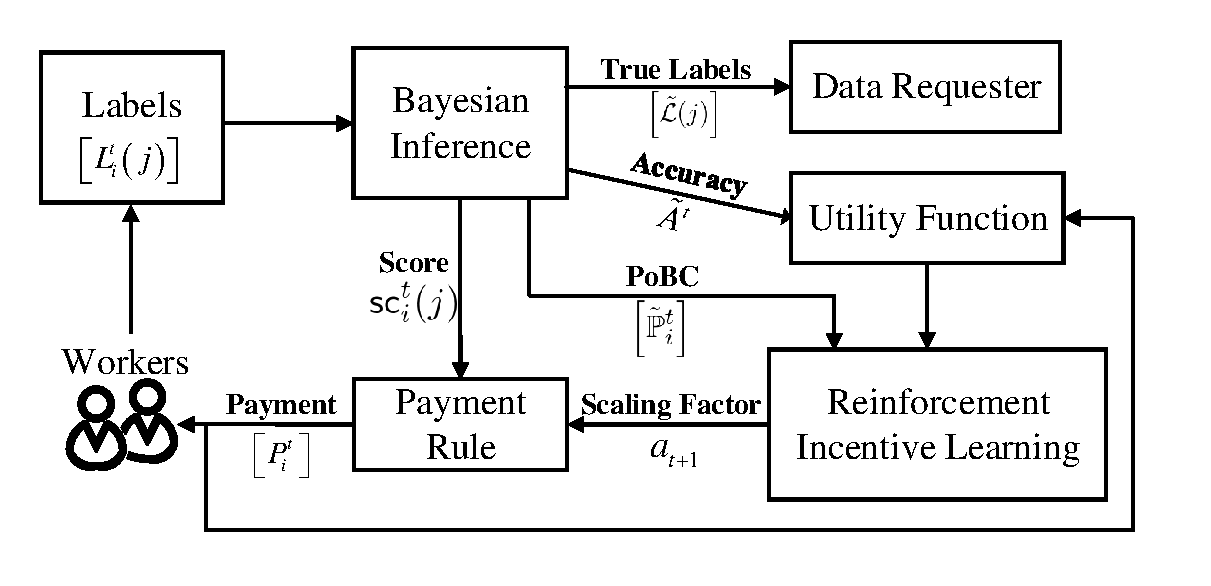
\includegraphics[width=0.48\textwidth]{image/Architecture}
	\vspace*{-8mm}
    \caption{\label{figure:layout} Layout of our incentive mechanism.}
\end{figure}
\section{Incentive Mechanism for Crowdsourcing}
Our mechanism mainly consists of three components: payment rule, Bayesian inference and reinforcement incentive learning (RIL); see Figure~\ref{figure:layout} for the overall layout, where estimated values are denoted with over-the-head tildes. 

 The payment rule ensures that reporting truthfully and exerting high efforts is the payment-maximizing strategy for all workers at any given time. Besides, our incentive mechanism as a whole guarantees that this is also the payment-maximizing strategy for all workers in the long-run. We kindly refer readers to Section~\ref{analysis} for the theoretical proof. This property prevents strategic manipulations from workers, which bring more long-term benefits to them by sacrificing short-term ones, or the other way around. 
By doing so, we wish to induce workers to generate high-quality labels. %and thus improve the label accuracy. 
The Bayesian inference algorithm is responsible for estimating the true labels, workers' PoBCs and the aggregate label accuracy from the collected labels at each time step. It utilizes soft Dirichlet priors and Gibbs sampling to prevent overestimation of accuracy when workers generate poor-quality labels. RIL adjusts the payment rule based on the historical data of payments, workers' PoBCs and aggregate labels' accuracy, aiming to optimally balance the utility gain from high accuracy and loss from large payments, which corresponds to $F(A^t)$ and $\sum_{i}P_i^t$ in Eqn.\ref{equation:utility} respectively. %In the following subsections, we provide a detailed formal introduction of the three one by one.

%Nevertheless, there are three challenges to achieve our design. Firstly, our empirical studies reveal that popular inference algorithms may be heavily biased towards overestimating the accuracy when the quality of labels is very low. For example, when there are $10$ workers and $q_i^t=0.55$, the estimated label accuracy of the EM estimator~\cite{dawid1979maximum,raykar2010learning} stays at around $0.9$ while the real accuracy is only around $0.5$.
%This heavy bias will cause the utility to be miscalculated and thus mislead our reinforcement adjustment.
%To reduce the inference bias, we develop our Bayesian inference algorithm by introducing the soft Dirichlet priors to both the true labels and workers' PoBCs.
%In this case, the posterior distribution cannot be expressed as any known distributions, which motivates us to derive the explicit posterior distribution at first and then employ Gibbs sampling to conduct inference.
%{\color{red}Secondly, the reinforcement adjustment expects the utility to be accurately calculated so that the direction of adjustment is clear.
%However, both the label accuracy and workers' PoBCs in our incentive mechanism are corrupted by noise.
%Considering that these estimates are calculated as an average over $M$ tasks, the central limit theorem ensures that the inference noise approaches the Gaussian distribution.
%Therefore, to overcome the inference noise, we develop our reinforcement adjustment algorithm based on the Gaussian process.}
%Lastly, the biggest challenge of our study is to prove that our incentive mechanism can ensure that reporting truthfully and exerting high efforts is the payment-maximizing strategy for workers in not only each time step and but also the long term.
%For clarity, we put the theoretical analysis in the next section.
%In this section, we focus on the first two challenges.


%Figure~\ref{Archi} shows the architecture of our incentive framework.
%Different from industrial feedback control systems, crowdsourcing markets require the data requester to announce the incentive mechanism to workers before allocating tasks to workers, which is actually a contract between two sides.
%So, we design our framework as two levels.
%The inner level is the Bayesian incentive mechanism which is always open to workers.
%Its objective is to ensure that reporting truthfully and exerting high efforts are the optimal strategy for all workers at any time step $t$.
%By doing so, we expect that all workers are fully rational and can follow this optimal strategy.
%However, in practice, human workers may not always fully rational and can even learn from the interactions with our mechanism.
%Thus, we develop the outer level, the reinforcement incentive mechanism, which adjusts the scaling level $a^t$ of our Bayesian mechanism to maximize the long-term utility of the data requester.
%Meanwhile, our reinforcement incentive mechanism must also ensure that reporting truthfully and exerting high efforts are the optimal strategy for workers in the long term.
%In this way, we can prevent the manipulation of any single worker.




\subsection{Payment Rule}
\label{payment}
To ensure IC (described in Section 5), we design the payment to worker $i$ for his/her label on task $j$ as
\begin{equation}
P^t_i(j)=a_t \cdot [\textsf{sc}^{t}_i(j)-0.5]+b
\label{equation:payment}
\end{equation}
where $\textsf{sc}^{t}_i(j)$ denotes worker $i$'s score on task $j$, which is calculated by our Bayesian inference algorithm. $b\geq 0$ is a constant representing the fixed base payment even if the worker purely genrates random labels. We use $a_t \in \mathcal{A}$ to denote the scaling factor, determined by RIL at the beginning of every step $t$. We assume $\mathcal{A}$ is a finite set.


\subsection{Bayesian Inference}
\label{inference}
%An accurate inference algorithm, which is responsible for estimating $L^{t}(j)$, $p^t_i$ and $A^t$, is the foundation of our framework. There have been many inference algorithms developed in the literature~\cite{zheng2017truth}. Among them, two popular ones are the EM estimator~\cite{dawid1979maximum} and the variational inference estimator~\cite{liu2012variational}.
%However, our empirical studies in Figure~\ref{BIM1} reveal that these iterative estimators, which may converge to the local optimum, will be heavily biased when the quality of labels is very low.
%Thus, we employ the similar Dirichlet priors as the variation inference estimator but explicitly derive the posterior distribution of true labels rather than relying on the evidence lower bound~\cite{blei2017variational}.
%Then, we use Gibbs sampling to efficiently sample the posterior distribution to calculate the estimates of $L^{t}(j)$, $p^t_i$ and $A^t$.

%since the EM estimator may converge to the local optimum.
%On the other hand, sampling-based Bayesian inference algorithms, for example Gibbs sampling, are computationally very expensive, even though they use the explicit posterior distribution and can avoid the inference bias.
%Especially, workers' scores are continuous variables, which will significantly slow down the convergence speed.
%Therefore, to the best of my knowledge, sampling-based Bayesian inference is never used for crowdsourcing where the number of workers and tasks is usually very large.
%In this section, to reduce the inference bias and meanwhile avoid overly large computation costs, we firstly assume Dirichlet priors for those continuous variables in our system and derive a joint posterior distribution which only contains the discrete variables.
%Then, we use Gibbs sampling to sample the obtained posterior distribution and estimate workers' scores based on those samples.

%\footnote{In practice, $M^{t}_{i}$ is often smaller than $M$, and we can introduce $L^{t}_i(j)=0$ to denote that task $j$ is not assigned to worker $i$. The incentive mechanisms developed in this paper can work well in the case where the matrix $[L^{t}_i(j)]$ is sparse. However, to simplify the theoretical analysis, we assume $M^{t}_{i}\equiv M$ in this paper and put the theoretical analysis on the sparse case as our future work.}

%In this subsection, we present the details of our inference algorithm.
For the simplicity of notations, we omit the superscript $t$ in this subsection. 
Before designing our own Bayesian inference algorithm, we ran several preliminary experiments using the existing inference algorithms popularly used by others. Our empirical studies reveal that those popular ones may be heavily biased towards overestimating the accuracy when the quality of labels is very low. For example, when there are $10$ workers and $\mathbb{P}^t_i=0.55$, the estimated label accuracy of the EM estimator~\cite{dawid1979maximum,raykar2010learning} stays at around $0.9$ while the real accuracy is only around $0.5$.\footnote{See Appendix H in Supplementary for details} This heavy bias will lead the data requester's utility $r^t$ to be miscalculated, causing two bad consequences. First, it induces bad incentive property, as workers with poor labelling accuracy now enjoy good estimates and thus high payments. Secondly, this potentially misleads RIL, as $r^t$ is used as reward. 

To reduce the inference bias, we develop our Bayesian inference algorithm by introducing soft Dirichlet priors to both the distribution of true labels $\bm{\tau}=[\tau_1,\tau_2]\sim \textrm{Dir}(\beta_{1},\beta_{2})$, where $\tau_1$ and $\tau_2$ denote that of label $1$ and $2$, respectively,  and workers' PoBCs  $[\mathbb{P}_{i}, 1-\mathbb{P}_i]\sim \textrm{Dir}(\alpha_{1},\alpha_{2})$. After doing so, we derive the conditional distribution of true labels given collected labels as (see Appendix I in Supplementary for detailed derivation)
%However, after doing so, the posterior distribution cannot be expressed as any known distributions, which motivates us to derive the explicit posterior distribution first and then employ Gibbs sampling to conduct inference.
%
%% For the simplicity of notations, we omit the superscript $t$ in this subsection.  %This heavy bias will cause the utility to be miscalculated and thus mislead our reinforcement adjustment.
%It is not had to figure out the joint distribution of the collected labels $\bm{L}$ and the true labels $\mathcal{L}$ 
%\begin{equation*}
%\label{JointDist}
%\begin{split}
%    &\mathbb{P}(\bm{L}, \mathcal{L}| \bm{\theta}, \bm{\tau})=\\ &\qquad {\prod}_{j=1}^{M}{\prod}_{k=1}^{2}\left\{\tau_{k}\prod_{i=1}^{N}\mathbb{P}_i^{\delta_{ijk}}(1-\mathbb{P}_i)^{\delta_{ij(3-k)}} \right\}^{\xi_{jk}}
%\end{split}
%\end{equation*}
%where $\bm{\theta}=[\mathbb{P}_1,\ldots, \mathbb{P}_N]$ and $\bm{\tau}=[\tau_1,\tau_2]$. $\tau_1$ and $\tau_2$ denote the distribution of true label $1$ and $2$, respectively.
%Besides,  $\delta_{ijk}=\mathbbm{1}(L_i(j)=k)$ and $\xi_{jk}= \mathbbm{1}(\mathcal{L}(j)=k)$.
%Here, we assume Dirichlet priors $\textrm{Dir}(\cdot)$ for $\mathbb{P}_i$ and $\bm{\tau}$, namely, 
%$
%[\mathbb{P}_{i}, 1-\mathbb{P}_i]\sim \textrm{Dir}(\alpha_{1},\alpha_{2}), \bm{\tau}\sim \textrm{Dir}(\beta_{1},\beta_{2}).
%$
%Then, the joint distribution of $\bm{L}$ and $\mathcal{L}$ satisfies
%\begin{equation*}
%\label{JointDist2}
%\mathbb{P}(\bm{L},\mathcal{L})={\int}_{\bm{\theta},\bm{\tau}}\mathbb{P}(\mathcal{L},\bm{L}|\bm{\theta}, \bm{\tau})\cdot \mathbb{P}(\bm{\theta}, \bm{\tau})\mathrm{d}\bm{\theta}\mathrm{d}\bm{\tau}.
%\end{equation*}
%Following Bayes' theorem, we derive the following
\begin{equation}
\label{PostDist}
\mathbb{P}(\mathcal{L}|\bm{L})=\mathbb{P}(\bm{L},\mathcal{L})/\mathbb{P}(\bm{L})\propto B(\hat{\bm{\beta}}){\prod}_{i=1}^{N}B(\hat{\bm{\alpha}}_{i}) 
\end{equation}
%
%\begin{equation}
%\label{JointDist2}
%\begin{split}
%&P(\mathcal{L},\bm{L},\bm{p}, \bm{\tau}|\bm{\alpha}, \bm{\beta})=P(\mathcal{L},\bm{L}|\bm{p}, \bm{\tau})\cdot P(\bm{p}, \bm{\tau}|\bm{\alpha}, \bm{\beta})\\
%&=\frac{1}{B(\bm{\beta})}\prod_{k=1}^{K}\tau_k^{\hat{\beta}_k-1}\cdot\prod_{i=1}^{N}\frac{1}{B(\bm{\alpha})}p_i^{\hat{\alpha}_{i1}-1}(1-p_i)^{\hat{\alpha}_{i2}-1}
%\end{split}
%\end{equation}
where $B(x,y)=(x-1)!(y-1)!/(x+y-1)!$ denotes the beta function, $\hat{\bm{\alpha}}=[\hat{\alpha}_1,\hat{\alpha}_2]$, $\hat{\bm{\beta}}=[\hat{\beta}_1,\hat{\beta}_2]$ and
\begin{equation*}
\begin{split}
&\hat{\alpha}_{i1}={\sum}_{j=1}^{M}{\sum}_{k=1}^{K}\delta_{ijk}\xi_{jk}+2\alpha_{1}-1\\
&\hat{\alpha}_{i2}={\sum}_{j=1}^{M}{\sum}_{k=1}^{K}\delta_{ij(3-k)}\xi_{jk}+2\alpha_{2}-1\\
&\hat{\beta}_k={\sum}_{j=1}^{M}\xi_{jk}+2\beta_{k}-1
\end{split}
\end{equation*}
where $\delta_{ijk}=\mathbbm{1}(L_i(j)=k)$ and $\xi_{jk}= \mathbbm{1}(\mathcal{L}(j)=k)$. The convergence of our inference algorithm requires $\alpha_1>\alpha_2$.
To simplify the theoretical analysis, we set $\alpha_1=1.5$ and $\alpha_2=1$ in the rest of this paper.
%\begin{equation}
%\begin{split}
%&\hat{\alpha}^{t}_{i1}={\sum}_{j=1}^{M}{\sum}_{k=1}^{K}\delta^{t}_{ijk}\xi^{t}_{jk}+\alpha_{1}\\
%&\hat{\alpha}^{t}_{i2}={\sum}_{j=1}^{M}{\sum}_{k=1}^{K}\delta^{t}_{ij(3-k)}\xi^{t}_{jk}+\alpha_{2}\\
%&\hat{\beta}^{t}_k={\sum}_{j=1}^{M}\xi^{t}_{jk}+\beta_{k}.
%\end{split}
%\end{equation}
%Besides, $B(x,y)=(x-1)!(y-1)!/(x+y-1)!$ denotes the beta function.
%The convergence of our inference algorithm requires $\alpha_1>\alpha_2$.
%To simplify the theoretical analysis, we set $\alpha_1=1.5$ and $\alpha_2=1$ in this paper.
%Meanwhile, we employ the uniform distribution for $\bm{\tau}$ by setting $\beta_1=\beta_2=1$.
%In this case, we can conduct marginalization via integrating Equation~\ref{JointDist2} over $\bm{p}$ and $\bm{\tau}$ as
%\begin{equation}
%\label{marginalization}
%\begin{split}
%P(\mathcal{L},\bm{L}|\bm{\alpha}, \bm{\beta})=\frac{B(\hat{\bm{\beta}})}{B(\bm{\beta})}\cdot {\prod}_{i=1}^{N}\frac{B(\hat{\bm{\alpha}}^{*}_{i})}{[B(\bm{\alpha})]^2}
%\end{split}
%\end{equation}
%where $\hat{\bm{\alpha}}^{*}_i=[\hat{\alpha}_{i1}+0.5,\hat{\alpha}_{i2}]$ and $\hat{\bm{\beta}}=[\hat{\beta}_1,\hat{\beta}_2]$. Following Bayes' theorem, we can know that
%\begin{equation}
%\label{PostDist}
%P(\bm{L}|\mathcal{L})=\frac{P(\mathcal{L},\bm{L}|\bm{\alpha}, \bm{\beta})}{P(\mathcal{L}|\bm{\alpha}, \bm{\beta})}\propto B(\hat{\bm{\beta}})\prod_{i=1}^{N}B(\hat{\bm{\alpha}}^{*}_{i}). 
%\end{equation}

%\begin{algorithm}[tb]
%   \caption{Gibbs sampling for crowdsourcing}
%   \label{GSC}
%   \small
%\begin{algorithmic}[1]
%   \vspace{0.5mm}
%   \STATE {\bfseries Input:} the collected labels $\bm{L}$, the number of samples $W$
%   \STATE {\bfseries Output:} the sample sequence $\mathcal{S}$
%   \vspace{0.5mm}
%   \STATE $\mathcal{S}\leftarrow\emptyset$, Initialize $\mathcal{L}$ with the uniform distribution
%   \FOR{$s=1$ {\bfseries to} $W$}
%   \FOR{$j=1$ {\bfseries to} $M$}
%   \STATE $\mathcal{L}(j) \leftarrow 1$ and compute $x_1= B(\hat{\bm{\beta}})\prod_{i=1}^{N}B(\hat{\bm{\alpha}}_{i})$
%   \STATE $\mathcal{L}(j) \leftarrow 2$ and compute $x_2= B(\hat{\bm{\beta}})\prod_{i=1}^{N}B(\hat{\bm{\alpha}}_{i})$
%   \STATE $\mathcal{L} \leftarrow$ Sample $\{1,2\}$ with $P(1)=x_1/(x_1+x_2)$
%   \ENDFOR
%   \STATE Append $\tilde{\mathcal{L}}$ to the sample sequence $\mathcal{S}$
%   \ENDFOR
%\end{algorithmic}
%\end{algorithm}

\begin{algorithm}[tb]
   \caption{Gibbs Sampling for Our Bayesian Inference}
   \label{GSC}
   \small
\begin{algorithmic}[1]
   \vspace{0.5mm}
   \STATE {\bfseries Input:} the collected labels $\bm{L}$, the number of samples $W$
   \STATE {\bfseries Output:} the sample sequence $\mathcal{S}$
   \vspace{0.5mm}
   \STATE $\mathcal{S}\leftarrow\emptyset$, Initialize $\tilde{\mathcal{L}}$ with the uniform distribution
   \FOR{$s=1$ {\bfseries to} $W$}
   \FOR{$j=1$ {\bfseries to} $M$}
   \STATE Compute $\mathbb{P}[\mathcal{L}(j)=k]$ by letting $\mathcal{L}(-j)=\tilde{\mathcal{L}}(-j)$.
   \STATE $\tilde{\mathcal{L}}(j) \leftarrow$ Sample $\{1,2\}$ with $\mathbb{P}[\mathcal{L}(j)=k]$
   \ENDFOR
   \STATE Append $\tilde{\mathcal{L}}$ to the sample sequence $\mathcal{S}$
   \ENDFOR
\end{algorithmic}
\end{algorithm}

Note we cannot derive an explicit formula for the distribution of a specific task $j$'s ground-truth from the conditional posterior distribution $\mathbb{P}(\mathcal{L}|\bm{L})$. We thus resort to Gibbs sampling for the inference.
More specifically, according to Bayes' theorem, we know that the conditional distribution of task $j$'s ground-truth $\mathcal{L}(j)$ satisfies
$\mathbb{P}[\mathcal{L}(j)|\bm{L}, \mathcal{L}(-j)]\propto \mathbb{P}(\mathcal{L}|\bm{L})$, where $-j$ denotes all tasks excluding $j$.
Leveraging this, we generate samples of the true label vector $\mathcal{L}$ following Algorithm~\ref{GSC}.
At each step of the sampling procedure (line 6-7), Algorithm~\ref{GSC} calculates $\mathbb{P}[\mathcal{L}(j)|\bm{L}, \mathcal{L}(-j)]$ first and then generates a new sample of $\mathcal{L}(j)$ to replace the old one in $\tilde{\mathcal{L}}$.
After traversing through all tasks, Algorithm~\ref{GSC} generates a new sample of the true label vector $\mathcal{L}$.
Repeating this process for $W$ times, we get $W$ samples, which is recorded in $\mathcal{S}$.
Here, we write the $s$-th sample as $\tilde{\mathcal{L}}^{(s)}$.
Since Gibbs sampling requires a burn-in process, we discard the first $W_0$ samples in $\mathcal{S}$. After doing so, we calcualte worker $i$'s score on task $j$ as
\begin{equation}
\label{equaton:score}
\textsf{sc}^{t}_i(j) = {\sum}_{s=W_0+1}^{W}\mathbbm{1}(\tilde{\mathcal{L}}^{(s)}(j)=L_{i}(j))/(W-W_0)
\end{equation}
and estimate worker $i$'s PoBC $\mathbb{P}_i$ as
\begin{equation}
\label{equation:p_infer}
\tilde{\mathbb{P}}_{i}=\frac{\sum\limits_{s=W_0+1}^{W}\left[2\alpha_{1}-1+\sum\limits_{j=1}^{M}\mathbbm{1}(\tilde{\mathcal{L}}^{(s)}(j)=L_{i}(j))\right]}{(W-W_0)\cdot(2\alpha_{1}+2\alpha_{2}-2+m_i)}
\end{equation}
and the distribution of true labels $\bm{\tau}$ as
\begin{equation}
\label{tau_infer}
\tilde{\tau}_{k}=\frac{\sum\limits_{s=W_0+1}^{W}\left[2\beta_{1}-1+\sum\limits_{j=1}^{M}\mathbbm{1}(\tilde{\mathcal{L}}^{(s)}(j)=k)\right]}{(W-W_0)\cdot(2\beta_{1}+2\beta_{2}-2+m_i)}.
\end{equation}
Furthermore, we define the log-ratio of task $j$ as
\begin{equation}
\label{ProbRatio}
\tilde{\sigma}_j=\log\frac{\mathbb{P}[\mathcal{L}(j)=1]}{\mathbb{P}[\mathcal{L}(j)=2]}=\log\left(\frac{\tilde{\tau}_1}{\tilde{\tau}_2}\prod_{i=1}^{N}\tilde{\lambda}_i^{\delta_{ij1}-\delta_{ij2}}\right)
\end{equation}
where $\tilde{\lambda}_i = \tilde{\mathbb{P}}_i/(1-\tilde{\mathbb{P}}_i)$.
Finally, we decide the true label estimate $\tilde{\mathcal{L}}(j)$ as $1$ if $\tilde{\sigma}_j>0$ and as $2$ if $\tilde{\sigma}_j<0$.
Correspondingly, the label accuracy $A$ is estimated as
\begin{equation}
\label{vot}
\begin{split}
\tilde{A}=\mathbb{E}\left(A \right) = \frac{1}{M}{\sum}_{j=1}^{M}e^{|\tilde{\sigma}_j|}\left(1+e^{|\tilde{\sigma}_j|}\right)^{-1}.
\end{split}
\end{equation}
For good inference accuracy, we require both $W$ and $W_0$ to be large values, and in the rest of this paper, we set $W=1000$ and $W_0=100$ respectively.
%Besides, compared the sampling-based inference which directly uses the joint distribution in Equation~\ref{JointDist}, the marginalization operation in Equation~\ref{marginalization} helps us to eliminate all the continuous variables, which can significantly boost the computation efficiency.
%Also, it is worth mentioning that, for the simplicity of notations, we omit the superscript $t$ in all the equations above.

\subsection{Reinforcement Incentive Learning}
\label{RL}
In this subsection, we formally introduce RIL, which adjusts the scaling factor $a^t$ at each time step $t$. Viewed under the big picture, it serves as the glue to connect each other component in our mechanism (see the edges and parameters around RIL in Figure~\ref{figure:layout}). To fully understand the technical fruit, we require the readers to at least be familiar with Q-value and function approximation. For readers with limited knowledge, we kindly refer them to Appendix A, where we provide a tutorial on these concepts.

With some transformation, the  crowdsourcing problem we aim to tackle in this paper can perfectly fit into the commonly used RL formalization (i.e. a Markov Decision Process). To be more specific, the data requester is the agent and it interacts with workers (i.e. the environment); scaling factors are actions; the utility of the data requester $r^t$ after paying workers (see Eqn.~\ref{equation:utility}) is the reward; how workers respond to different incentives and potentially change their internal states thereafter forms the transition kernel, which is unobservable; what scaling factor to be picked at each step $t$ given workers' labelling constructs the policy, which needs to be learned. Note that, since the real accuracy cannot be observed, we use the estimated accuracy $\tilde{A}$ calculated by Eqn.\ref{vot} instead to construct the reward
\vspace{-2mm}
\begin{equation}
\label{equation:approx_reward}
r_t\approx F(\tilde{A}^t) - \eta {\sum}_{i=1}^{N}P^t_i.
\end{equation}

\vspace{-2mm}
To achieve better generalization across different states, it is a common approach to learn a feature-based state representation $\phi(s)$ \citep{Mnih15, Liang16}. Recall that the data requester's implicit utility at each time $t$ only depends on the aggregate PoBC averaged across the whole worker body. Such observation already points out to a  representation design with good generalization, namely 
$\phi(s_t) = {\sum}_{i=1}^N \mathbb{P}^t_i/N$.
Further recall, when deciding the current scaling factor $a_t$, the data requester does not observe the latest workers' labelling and thus cannot directly estimate the current $\phi(s_t)$ via Bayesian inference. Due to this one-step delay, we have to build our state representation using the previous observation. Since most workers would only change their internal states after receiving a new incentive, there exists some imperfect mapping function $\phi(s_{t}) \approx f(\phi(s_{t-1}),a_{t-1})$. %Putting into another perspective, the combination of $\phi(s_{t-1})$ and $a_{t-1}$ also reflects our best knowledge of the current state. 
Utilizing this implicit function, we introduce the augmented state representation in RIL
$$\hat{s}_t = \langle \phi(\hat{s}_{t-1}), a_{t-1} \rangle.$$

%Since the data requester never possesses the ground-truth for each task, the utility $u^t$ is not accurately observed. Also note $\hat{s}_t$ is hardly perfectly accurate. % as the mapping function can not be perfect. 
%Combining both together,
\vspace{-2mm}
Since neither $r_t$ nor $\hat{s}_t$ can be perfectly accurate, it would not be a surprise to observe some noise that cannot be directly learned in our Q-function. %Recall Eqn.~\ref{vot} shows that the estimated accuracy is calculated as an average across all $M$ tasks. 
As for most crowdsourcing problems the number of tasks $M$ is large, we leverage the central limit theorem to justify our modeling of the noise using a Gaussian process.
To be more specific, we calculate the temporal difference (TD) error as 
\begin{equation}
r_t \approx Q^\pi(\hat{s}_t, a_t) - \gamma \mathbb{E}_{\pi}Q^{\pi}(\hat{s}_{t+1},a_{t+1}) + \epsilon_t 
\end{equation}
where the noise $\epsilon $ follows a Gaussian process $\mathcal{N}(\hat{s}_t,\hat{s}_{t+1})$, and $\pi=\mathbb{P}(a|\hat{s})$ denotes the current policy.
 Doing so, we gain two benefits. First, it greatly simplifies the derivation of the update for the Q-function. Secondly, as shown in our empirical results later, it is robust under different worker models.
Besides, following \citet{gasic2014gaussian} we approximate Q-function as
$$
Q^{\pi}(\hat{s}_{t+1},a_{t+1})\approx\mathbb{E}_{\pi}Q^{\pi}(\hat{s}_{t+1},a_{t+1})+\epsilon_{\pi}
$$
where $\epsilon_{\pi}$ also follows a Gaussian process.
%when studying the dialogue with human beings, \citet{gasic2014gaussian} has demonstrated a notably successful approximation of Q-function by letting $Q^{\pi}(\hat{s}_{t+1},a_{t+1})\approx\mathbb{E}_{\pi}Q^{\pi}(\hat{s}_{t+1},a_{t+1})+\epsilon_{\pi}$, where the noise $\epsilon_{\pi}$ also follows a Gaussian process.
%To analyze how human workers response to incentives, we also employ this approximation technique when developing our algorithm.

Under the Gaussian process approximation, all the observed rewards and the corresponding $Q$ values up to the current step $t$ form a equation set, and it can be written as
\begin{equation}
\bm{r}=\bm{H}\bm{Q}+\bm{N}
\end{equation}
where $\bm{r}$, $\bm{Q}$ and $\bm{N}$ denote the collection of rewards, $Q$ values, and residuals. Following Gaussian process's assumption for residuals, $\bm{N}\sim \mathcal{N}(\bm{0},\bm{\sigma}^2)$, where $\bm{\sigma}^2=\textrm{diag}(\sigma^2,\ldots,\sigma^2)$.
The hat matrix $\bm{H}$ satisfies $\bm{H}(k,k)=1$ and $\bm{H}(k,k+1)=-\gamma$ for $k=1,\ldots, t$.
Then, by using the online Gaussian process regression algorithm~\cite{engel2005reinforcement}, we effectively learn the Q-function as
\begin{equation}
\label{equation:update}
Q(\hat{s},a) = \bm{k}(\hat{s},a) ^{\mathrm{T}}(\bm{K} +\bm{\sigma}^2)^{-1}\bm{H}^{-1}\bm{r}
\end{equation}
where $\bm{k}(\hat{s},a)=[k((\hat{s},a), (\hat{s}_1,a_1)),\ldots, k((\hat{s},a), (s_t,a_t))]^{\mathrm{T}}$ and $\bm{K}=[\bm{k}(\hat{s}_1,a_1),\ldots,\bm{k}(\hat{s}_t,a_t)]$. Here, we use $k(\cdot, \cdot)$ to denote the Gaussian kernel.
Finally, we employ the classic $\epsilon$-greedy method to decide $a_t$ based on the learned Q-function.
To summarize, we provide a formal description about our RL algorithm in Algorithm~\ref{RAC}. Note that, when updating $\bm{K}$, $\bm{H}$ and $\bm{r}$ in line 6, we employ the sparse approximation to discard some data so that the size of these matrices will not increase finitely. The details of this technique can be found in \citet{gasic2014gaussian}.

\begin{algorithm}[tb]
   \caption{Reinforcement Incentive Learning (RIL)}
   \label{RAC}
   \small
\begin{algorithmic}[1]
   \FOR{each episode}
   \FOR{each step in the episode}
   \STATE Decide the scaling factor as ($\epsilon$-greedy method)
   			\vspace{-3mm}
			$$\ \ a_t=\left\{
			\begin{array}{ll}
				\arg\max_{a\in\mathcal{A}}Q(\hat{s}_t,a) & \mathrm{Probability\ } 1-\epsilon\\
				\mathrm{Random\ } a\in\mathcal{A} & \mathrm{Probability\ } \epsilon
			\end{array}						
			 \right.$$  
			 \vspace{-3mm} 
   \STATE Assign tasks and collect labels from the workers
   \STATE Run Bayesian inference to get $\hat{s}_{t+1}$ and $r_t$
   \STATE Use $(\hat{s}_t, a_t, r_t)$ to update $\bm{K}$, $\bm{H}$ and $\bm{r}$ in Eqn.\ref{equation:update}
   \ENDFOR
   \ENDFOR
\end{algorithmic}
\end{algorithm}

% Due to the fact that in most crowdsourcing problems the number of workers is limited to be fewer than thousands, we decide to design a high-quality human-engineered static feature representation for our RL algorithm. Note though recently because of deep RL's huge success, static feature representation has been less popular, its competitiveness is demonstrated even in the most challenging domains \citep{Mnih15,Liang16}.

%Besides, presented as the layout of our mechanism, Figure~\ref{figure:layout} also visualizes how our RL algorithm interacts with the environment and the rest of the framework;  it takes as input workers' PoBC, reward signal, and internally its action history, and outputs the next-step scaling factor.
%
%%The latest determined scaling factor gets plugged back into the payment rule, and by following Eqn.\ref{equation:payment}, the exact payment to each worker is then decided.  
%

 
%As a critical step towards improving a given policy, it is a standard practice for RL algorithms to learn a state-action value function (i.e. Q-function), denoted:
%\begin{equation*}
%\begin{split}
%&Q^\pi(s,a) =\\
%& \quad\mathbb{E}\left[ \mathcal{R}(s_t,a_t,s_{t+1}) + \gamma V^\pi(s_{t+1}) \mid s_t = s, a_t = a \right].
%\end{split}
%\end{equation*}
%In real-world problems, in order to achieve better generalization, instead of learning a value for each state-action pair, it is more common to learn an approximate value function: $Q^\pi(s,a; \theta) \approx Q^\pi(s,a)$. A standard approach is to learn a feature-based state representation $\phi(s)$ instead of using the raw state $s$. Due to the popularity of Deep Reinforcement learning, it has been a trend to deploy neural networks to automatically extract high-level features \citep{Silver17,Mnih15}. 
%However, most deep RL methods' success is only demonstrated in domains where the environment is very high-dimensional \citep{}. Unfortunately, this prerequisite does not hold in most crowdsourcing problems, where the number of workers are limited to be fewer than thousands. Due to this fact, we turn our attention to designing a high-quality human-engineered feature representation, which embodies our knowledge of this domain. Several studies also reveal that a carefully designed static feature representation can achieve performance as good as the most sophisticated state-of-the-art deep RL models, even in the most challenging domains \citep{Liang16}.
%
%Recall that the data requester's implicit utility at each time $t$ only depends on the aggregate probability of being correct averaged across the whole worker body. Such observation already points out to a  representation design which guarantees good generalization. To be more specific, we construct our state representation as 
%$\phi(s_t) = \sum_{i=1}^N \mathbb{P}^t_i/N.$
%Further recall, when deciding the current scaling factor $a_t$, the data requester does not observe the latest workers' labelling and thus cannot directly estimate the current $\phi(s_t)$ via Bayesian inference. Due to this one-step delay, we have to build our state representation using the previous observation. Since most workers would only change their effort levels and reporting strategies after receiving a new incentive, there exists some imperfect mapping function $\phi(s_{t}) \approx f(\phi(s_{t-1}),a_{t-1})$. Putting into another perspective, the combination of $\phi(s_{t-1})$ and $a_{t-1}$ also reflects our best knowledge of the current state. Utilizing this implicit function, we formally introduce an augmented state representation for our RL algorithm
%$$
%\hat{s}_t = \langle \phi(s_{t-1}), a_{t-1} \rangle .
%$$
%Since the data requester never possesses the ground-truth for each task, the utility $u^t$ is not accurately observed. Also note $\hat{s}_t$ is hardly perfectly accurate. % as the mapping function can not be perfect. 
%Combining both together, it would not be a surprise to observe some noise that cannot be directly learned in our state-action value function. 
%
%
%Recall Eqn.~\ref{vot} shows that the estimated accuracy is calculated as an average across all $M$ tasks. 
%As for most crowdsourcing problems $M$ is a large number, we leverage the central limit theorem to justify our modelling of the noise using a Gaussian process.
%To be more specific, we calculate the temporal difference (TD) error as 
%$$
%r_t \approx Q^\pi(\hat{s}_t, a_t) - \gamma V^\pi(\hat{s}_{t+1}) + \epsilon_t $$
%where the noise $\epsilon $ follows a Gaussian process $\mathcal{N}(\hat{s}_t,\hat{s}_{t+1})$. Note we gain two benefits doing so. First, it greatly simplifies our derivation of the update for the Q-function. Secondly, our empirical results later show that this Gaussian approximation has achieved robust performance under different worker models.  
%
%Under the Gaussian process approximation, we can put all the observed rewards and the corresponding $Q$-function up to the current step $t$ together and obtain
%\begin{equation}
%\bm{r}=\bm{H}\bm{Q}+\bm{N}
%\end{equation}
%where $\bm{r}$, $\bm{Q}$ and $\bm{N}$ denote the collection of rewards, $Q$ values, and residual values up to step $t$, respectively.
%Due to the Gaussian process assumption of the residual, $\bm{N}\sim \mathcal{N}(\bm{0},\bm{\sigma}^2)$, where $\bm{\sigma}^2=\textrm{diag}(\sigma^2,\ldots,\sigma^2)$.
%The hat matrix $\bm{H}$ satisfies that $\bm{H}(k,k)=1$ and $\bm{H}(k,k+1)=-\gamma$ for $k=1,\ldots, t$.
%Then, by using the online Gaussian process regression algorithm~\cite{engel2005reinforcement}, we can effectively learn the Q-function as
%\begin{equation}
%\label{equation:update}
%Q(s,a) = \bm{k}(s,a) ^{\mathrm{T}}(\bm{K} +\bm{\sigma}^2)^{-1}\bm{H}^{-1}\bm{r}
%\end{equation}
%where $\bm{k}(s,a)=[k((s,a), (s_1,a_1)),\ldots, k((s,a), (s_t,a_t))]^{\mathrm{T}}$ and $\bm{K}=[\bm{k}(s_1,a_1),\ldots,\bm{k}(s_t,a_t)]$. Here, we use $k(\cdot, \cdot)$ to denote the Gaussian kernel.
%Furthermore, we use the classic $\epsilon$-greedy method to construct policy from the learned Q-function.
%To summarize, we provide a formal description about our reinforcement learning algorihtm in Algorithm~\ref{RAC}.
%Note that, when updating $\bm{K}$, $\bm{H}$ and $\bm{r}$ in line 6, we employ the sparse approximation to discard some historical data so that the size of these matrices and vectors will not increase finitely. The details of this approximation technique can be found in \citet{gasic2014gaussian}.
%
%\begin{algorithm}[tb]
%   \caption{RL Algorithm for Crowdsourcing}
%   \label{RAC}
%   \small
%\begin{algorithmic}[1]
%   \FOR{each episode}
%   \FOR{each step in the episode}
%   \STATE Decide the scaling factor as ($\epsilon$-greedy method)
%			$$\ \ a_t=\left\{
%			\begin{array}{ll}
%				\arg\max_{a\in\mathcal{A}}Q(\hat{s}_t,a) & \mathrm{Probability\ } 1-\epsilon\\
%				\mathrm{Random\ } a\in\mathcal{A} & \mathrm{Probability\ } \epsilon
%			\end{array}						
%			 \right.$$   
%   \STATE Assign tasks and collect labels from the workers
%   \STATE Run Bayesian inference to get $\hat{s}_{t+1}$ and $r_t$
%   \STATE Use $(\hat{s}_t, a_t, r_t)$ to update $\bm{K}$, $\bm{H}$ and $\bm{r}$ in Eqn.\ref{equation:update}
%   \ENDFOR
%   \ENDFOR
%\end{algorithmic}
%\end{algorithm}